\chapter{Information Theoretic Fuel Cycle Analysis}
\index{Information Theoretic Fuel Cycle Analysis@\emph{Information Theoretic Fuel Cycle Analysis}}
\label{cts_paper}



\section{Introduction}
\index{Introduction@\emph{Introduction}}
\label{cts_sec:intro}

Technology development and deployment (TD\&D) decisions will play a key role in
establishing the array of diverse, interconnected technologies that might comprise
future nuclear fuel cycles (NFCs).  These decisions are made in view of one or more
objectives for the NFC the technology will support.  Objectives include minimizing
electricity production costs, increasing the efficiency of resource or geologic
repository utilization, and mitigating the risk of safety incidents or misuse of
technologies or materials.

TD\&D decisions are justified by weighing their costs against the expected benefits,
monetary, monetizable or otherwise, that follow when they come to fruition.  To that
end, multiple NFC simulation models  \cite{Jacobson2009} \cite{GENIUS1} have been devised.  
One aim of these models is enable these hypothetical outcomes to be quantified.  Two major 
challenges associated with this goal are the uncertainties in the deployment and performance 
of other NFC technologies and the nuclear energy industry as a whole, and the complex 
interdependence between the technology being considered, other NFC technologies and their 
own (uncertain) characteristics, and NFC outcomes.

This paper addresses these challenges by applying entropy-based statistical methods of information
theory to describe outcomes produced by an NFC model.  Past efforts at sensitivity and uncertainty
analysis on this system have largely been limited to deterministic approaches.  For instance,
brute-force techniques of linear sensitivity analysis have been used to give rise to sensitivity
coefficients, i.e. the change in an outcome divided by the change in an input.  In principle, these
coefficients are valuable inputs to the TD\&D decision-making process since they can inform the
return on an investment.  For example, the incremental gain in heat-limited repository capacity per
unit change in the efficiency of separating, say, americium from used fuel.

However, the coefficients have a limited range of validity since they are departures from a
`base case' where each input is varied singly, holding others fixed.  Returning to the above example,
the gain in repository capacity might be found to be quite small if the separation efficiency
of plutonium is low (since Pu dominates the heat load borne by the repository). 
On the other hand the repository capacity gains would be large
if the Pu separation efficiency is high (and Am dominates the heat load).  Many other
parameter combinations of this type can be imagined, each contingent on and affecting 
the characteristics of one of the fuel cycle technologies.  Comprehensive,
brute-force evaluation of a parameter space of this size may not be feasible.

Since the system being simulated is complex, it is appropriate to treat it as a `black box'
and use statistical measures to characterize its behavior.  This paper subjects an NFC simulator
to a contingency table analysis, that in turn unlocks functional-form independent, entropy-based
measures of input-output dependence.  The contingency tables are generated by stochastically invoking
the NFC simulator; each scenario realization consists of thirty technology-defining inputs sampled
from distributions encompassing physically meaningful values.  Computed from the contingency tables,
the entropy statistic establishes the strength of correlation between any input and any output
without defining a `base case' or set of reference technology properties.

To capture joint sensitivities, like the simultaneous and complex interdependence of the
above-mentioned Pu and Am separation efficiencies on repository capacity, a novel statistical
measure is defined.  This measure, a coefficient of variation, uses three-dimensional contingency
table data to describe the change in the variance of an outcome with respect to one input, over the
range of admissible values of a second input.  A high value for this statistic indicates that the
impact of one input on the outcome is strongly dependent on the value of the second input.  This
measure supports fuel cycle analysis and TD\&D decision-making by identifying inputs (and their
parent technologies) that can, if also altered, augment or reduce the effect of the decision
being considered.

The remainder of this paper is organized as follows.  Section 2 begins with a summary of the
methodology employed to carry out the study.  Section 3 describes the fuel cycle simulations and 
method for sampling the input parameters to be varied, while section 4 presents the theoretical 
background underpinning the entropy-based
statistical measures.  Section 5 provides results for the statistical measures applied to the scenario
space outlined in Section 3 and offers several case studies that illustrate the interpretation
of the statistical outcomes.

\section{Methodology}
\index{Methodology@\emph{Methodology}}
\label{cts_sec:methodology}

Statistical performance measures are applicable to a nuclear fuel cycle simulation model that
is amenable to stochastic execution under variation of several independent parameters.  Values
for each input are to be chosen stochastically from a predefined, physically-valid range.
By generating many inputs and tabulating the corresponding results from an underlying physics-based
fuel cycle model, the fuel cycle undergoes a Monte Carlo simulation.  An input-output vector
constitutes a single fuel cycle realization.  From here, relevant statistical metrics on the set of
realizations yield information on how the system as a whole performs.  This methodology may be seen
graphically in Figure \ref{mcmethod}.

\begin{figure}[htbp]
\begin{center}
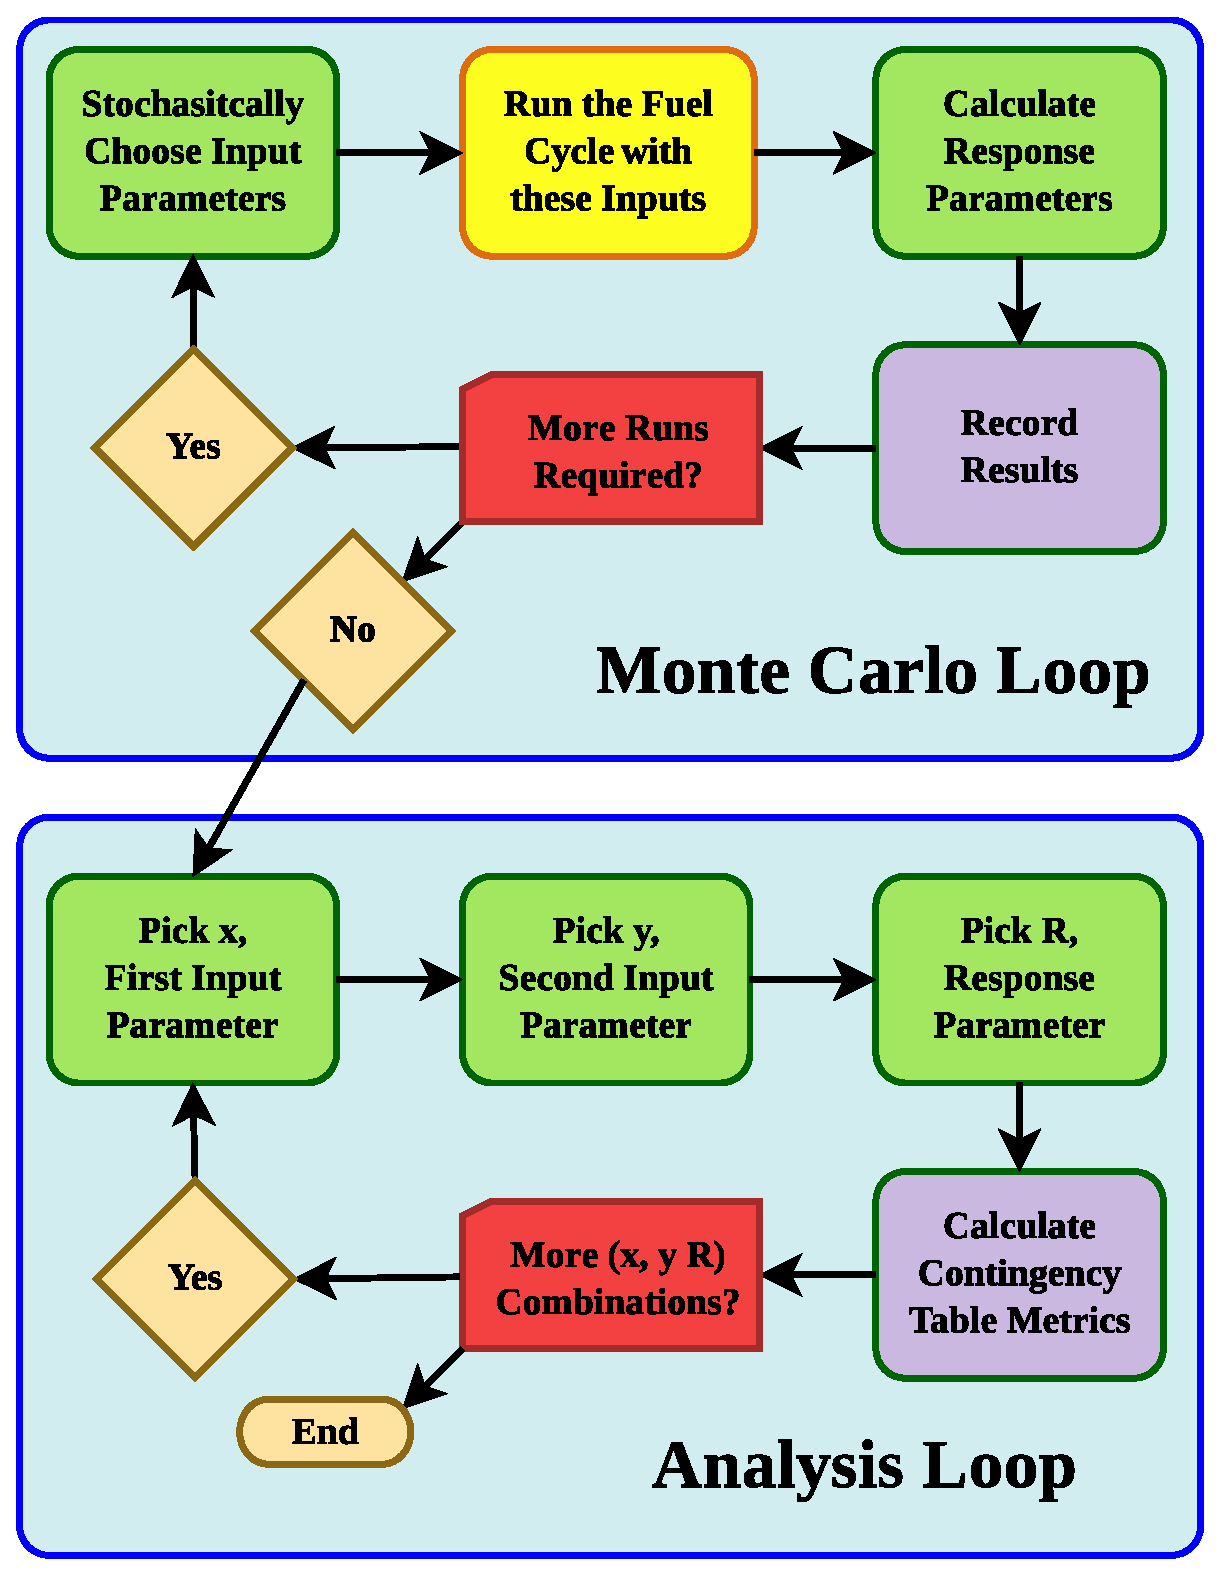
\includegraphics[scale=0.70]{ct_sensitivity/figs/MonteCarloMethodology.eps}
\caption{Monte Carlo Methodology \& Analysis Diagram}
\label{mcmethod}
\end{center}
\end{figure}

To further system analysis objectives, `standard' statistical metrics (such as the mean response
over all runs) may be calculated.  However, the usual correlation coefficients imply a linear
relationship between input and response.  Given the complexity of the system, linearity is not
a safe assumption for many system metrics.  Thus, novel information theoretic measures have
proved more valuable to ranking the importance of input parameters.

Additionally, it is useful to extend the information theoretic metrics from their typical 2D
formulations to the three dimensional equivalents.  If 3D metrics are constructed such that
they relate two input parameters to a response, then joint sensitivity or co-variance information
can be computed from a single set of stochastically-generated data.  Conditional covariances
(sensitivity of sensitivity) can thus be measured for two inputs to one response.
To maintain a realistic physical interpretation of this type of covariance, a combination of
entropy-based metrics extended to 3D metrics can be formulated  (discussed in section
\ref{sec:sensitivity_of_sensitivity_metrics}).  Any statistical analysis along these lines, though,
must be built around a model of the flow of materials through the nuclear fuel cycle, and the
transformations that constituent NFC technologies apply to the material flow.




\section{Nuclear Fuel Cycle Simulation}
\index{Nuclear Fuel Cycle Simulation@\emph{Nuclear Fuel Cycle Simulation}}
\label{cts_sec:nfcsim}

A fuel cycle simulation package that incorporates physics-based submodels of reactor burnup \cite{Scopatz2009} and
repository performance \cite{Li2009} served as the platform for this analysis. The approach taken in each
submodel is briefly summarized below. For additional details on this package refer to \cite{Li2009b}.

The importance of physics-based models (as opposed to curve fits or other parameterizations that are valid
only under specific conditions) in a sensitivity study of this type must be stressed. Given the number of
degrees of freedom associated with a fuel cycle scenario, it is not feasible, for example, to parameterize
reactor burnup with respect to transuranic isotopic stream compositions. Nor would it be possible to do
so for repository performance with respect to changes in host medium physical properties or system
geometry.

The reactor submodel couples burnup and criticality calculations \cite{Scopatz2009}. The burnup portion of the
model uses pre-tabulated physical data for each initially-present nuclide (neutron production and destruction
rates, burnup, and isotopic transformation) that are functions of fluence. These input curves are specific to a
given reactor and fuel type. The reactor model then uses mass-weighted superposition to recombine these
isotopic parameters as needed to calculate the multiplication factor and maximum discharge burnup. This result is
then folded in with a linear reactivity model for multi-batch criticality calculations that derive viable
fresh fuel compositions.

The repository thermal analysis model was developed based on the
analytical solution of a thermal conduction model for the presence of
loaded nuclear waste in a geologic repository \cite{Li2010a}. The
repository is modeled as a homogenous hosting medium with constant
properties. The nuclear waste packages were assumed to be loaded into parallel
waste emplacement drifts. Each drift is treated as
an infinite line heat source. The temperature increase at the critical
location is the superposition of temperature increase from each drift. The
undisturbed temperature field was assumed to be known, and the repository
capacity was determined according to the appropriate thermal design
constraints.



\subsection{Fuel Cycle Schema}
\index{@\emph{}}
\label{cts_sec:fcschema}

\begin{figure}[htbp]
\begin{center}
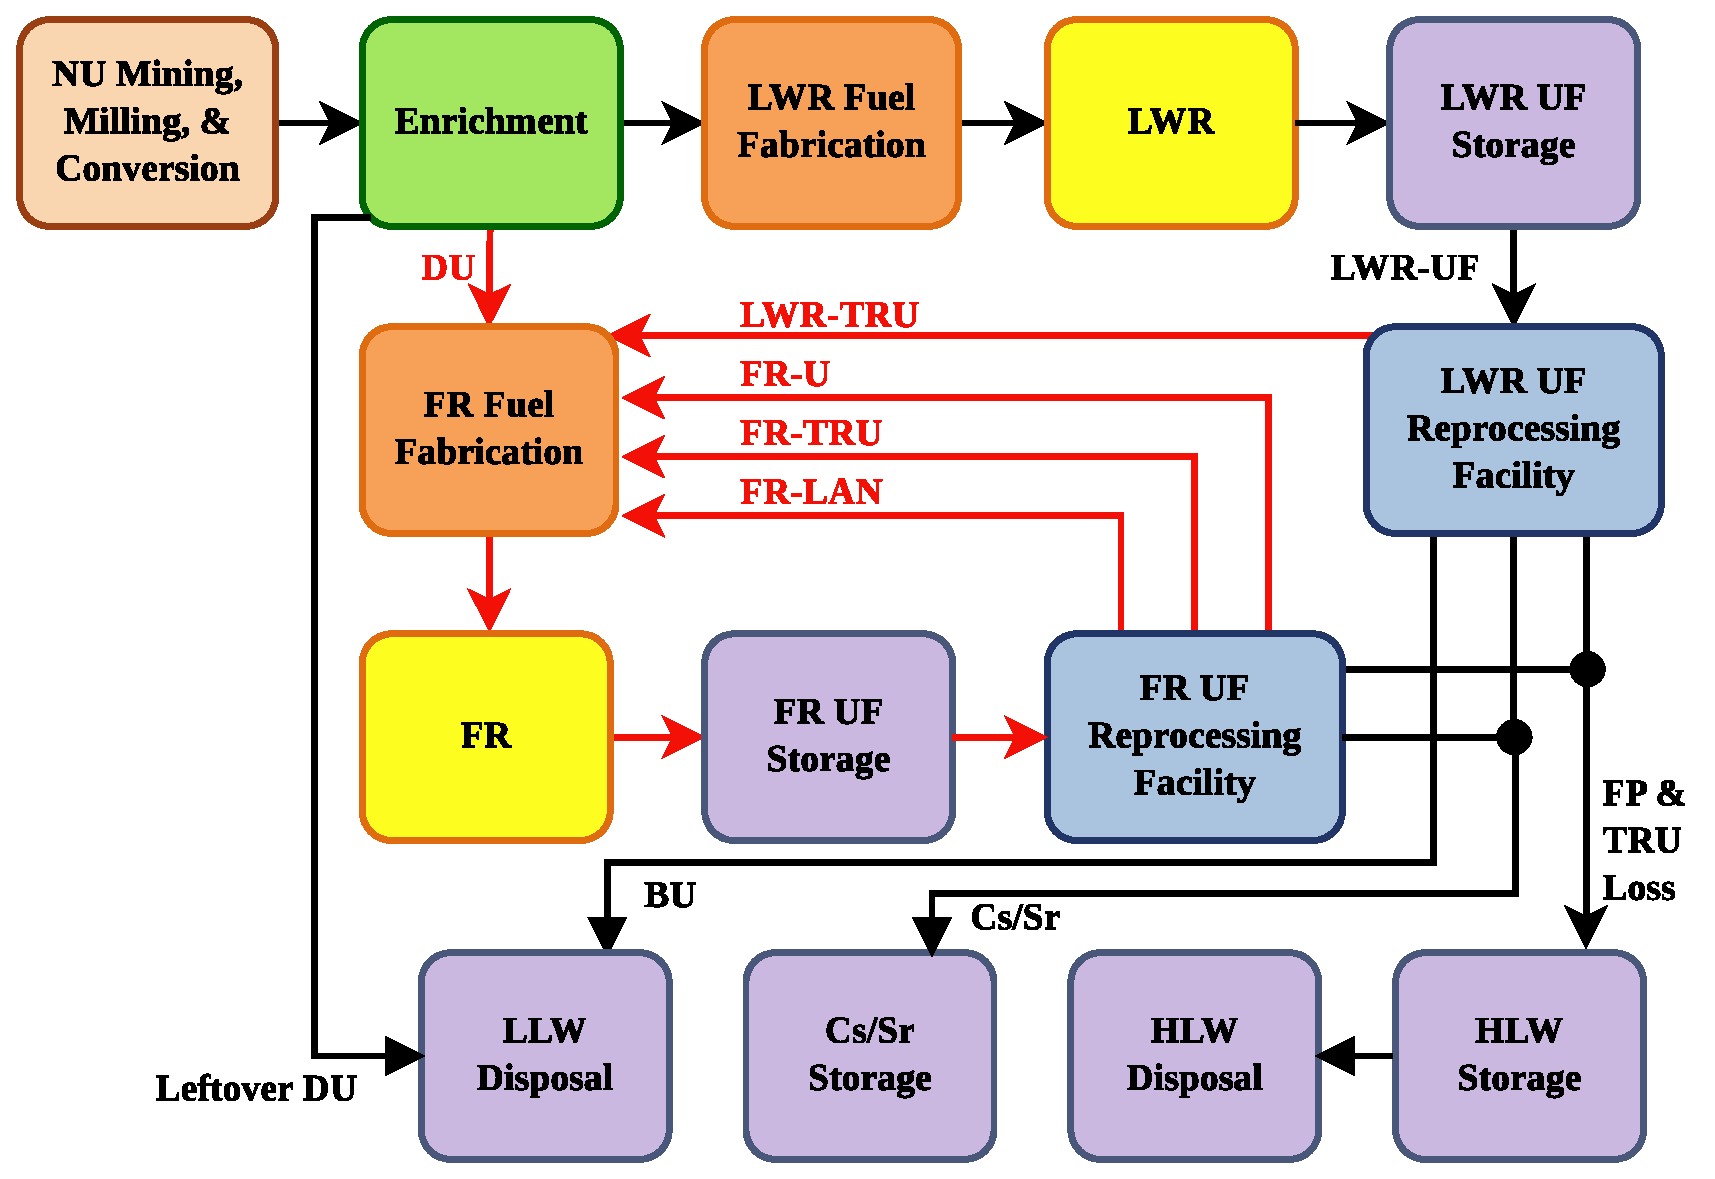
\includegraphics[scale=0.50]{figs/LWR_FR.eps}
\caption{LWR-FR Symbiotic Fuel Cycle Scenario}
\label{lwr_fr_fc}
\end{center}
\end{figure}

A sodium cooled fast burner (FR) - light water reactor (LWR) symbiotic cycle is studied here.
It is more fully detailed in \cite{Li2009b} and the corresponding flowchart
is seen in Figure \ref{lwr_fr_fc}. Although the model computes recycle passes
leading up to equilibrium \cite{Scopatz2009}, data (\emph{i.e.} the system wide performance
assessment metrics) are taken only after the fuel cycle has achieved its mass-balance equilibrium.
The statistical techniques discussed below could be applied to any type of fuel cycle; in this study,
the LWR and Na-cooled FR technologies were chosen for the fuel cycle simulation model
in order to strike a reasonable balance between input space richness, complexity, and familiarity to readers.

The fast reactors exist in support of the current and near-future
fleet of light-water reactors. The LWR used fuel (UF), after a cooling
period, is sent to an aqueous reprocessing facility. Here the transuranics (TRU) are separated out
from the fission products (FP) and
the burned uranium (BU).  The FP stream is further partitioned at the
LWR fuel reprocessing plant. The cesium and strontium are
separated out from the remaining FP. The Cs and Sr are
then emplaced in a storage facility built for medium-lived
isotopes while the BU goes to a low-level waste (LLW) disposal facility.
The remaining FPs and any losses from the other
streams (TRU, U, Cs/Sr) are treated as high-level waste (HLW) and sent to
the repository for permanent disposal.

Meanwhile, the recovered transuranics from the LWR
are mixed with depleted uranium (DU), and recycled FR
uranium and TRU. In this schema, all of the U and TRU
discharged from a FR (less reprocessing losses) are recycled into the fast reactor.
Thus the DU and LWR-TRU streams act as a top-up. By mixing in appropriate proportions (as
calculated in \cite{Scopatz2009}), new fuel for the fast reactors is
created.

After being re-burned in the FR, the used fuel once
again goes into cooling for three to thirty years. From here the fuel
is sent to a FR fuel reprocessing facility.  At the FR fuel reprocessing facility the actinide mass
of FR-UF is separated from the fission products present.
Again, the Cs and Sr are separated from the remaining FP.
The actinides are sent back to the fast reactor, the Cs/Sr
stream is disposed of in its own storage facility, and the
non-Cs/Sr fission products and losses from other streams
are sent to the deep geologic repository.  After reprocessing but prior to emplacement in the repository, the high level waste
stream is cooled for between one and three hundred years.
The deep geologic repository itself is modeled after
Yucca Mountain.



\subsection{Implementation}
\index{Implementation@\emph{Implementation}}
\label{cts_sec:implementation}

The fuel cycle model has been benchmarked against OECD and Idaho National Laboratory
(VISION) scenario analyses. When compared against the LWR-FR symbiotic cycle defined in Scheme
3a of the 2006 OECD fuel cycle system study \cite{NEA-5990}, agreement to within 5\% on the LWR-to-FR support
ratio and uranium and plutonium isotopics in the equilibrium mass flows was seen. Full benchmark
results are reported in \cite{Scopatz2009} and \cite{Li2009}.  For further details on this LWR-FR
symbiotic cycle refer to \cite{Shropshire2009}. The LWR and FR input parameters defined in
\cite{Shropshire2009} and reproduced in \cite{Scopatz2009} are points of departure for the
statistical analyses.

The physics-based methodology allows reactor performance and fuel cycle mass
balances to be rapidly recalculated under perturbations to design and operating parameters, where feedbacks to the operation of the cycle may have global reach.

\subsection{Parameter Specification}
\index{Parameter Specification@\emph{Parameter Specification}}
\label{cts_sec:paramspec}

Stochastic parameters are sampled either in a linearly uniform, log uniform, or one-minus-log uniform fashion.
The one-minus-log uniform distribution is useful for choosing separation efficiencies and is known as sampling
in the `nines'.  Table \ref{param_def} defines all thirty fuel cycle input parameters along with the six
responses computed by the model.  The scale column lists the sampling function
and the binning method implemented (see section \ref{sec:binning}) for each input parameter.

In the case where a set of input parameters is chosen such that the cycle is not physically calcuable,
internal variables inside of the models are adjusted to a point such that the fuel cycle is feasible.
For example, suppose a vector of inputs specifies a high value of the LWR burnup as well as other default
internal parameters.  The reactor model will adjust the non-leakage probability, the initial enrichment
of the fresh fuel, and the discharge fluence until these are tuned such that the stochastic burnup value
is obtained.

Thus every fuel cycle realization is its own distinct cycle, tuned for the stochastic parameters selected.
However, by bounding the input parameters and comparing many realizations, this study shows that the
output parameters are also bounded.  The spread of the output parameters due to changes in the inputs
determines the relative importance of that input.


%Input Variable Definition
\begin{table}
\caption{Fuel Cycle Parameter Definition}
\begin{center}
%\scriptsize
\tiny
\begin{tabular}{|l|l||c|c|c|c|}
\hline
\textbf{Input Parameter $x$} & \textbf{Abbreviation} & \textbf{Min} & \textbf{Max} & \textbf{Units} & \textbf{Scale}\\
\hline
LWR Burnup Level & \texttt{LWR\_BUd} & 30.0 & 80.0 & MWd/kgIHM & linear \\
\hline
LWR Fuel to Moderator Ratio & \texttt{LWR\_Fuel2Mod} & 0.28 & 0.36 & & linear \\
\hline
LWR UF Storage Time & \texttt{LWR\_UF\_Storage\_Time} & 3 & 30 & years & linear \\
\hline
SE of U from LWR UF & \texttt{LWR\_SE\_U} & 0.99 & 0.9999 & & nines \\
\hline
SE of NP from LWR UF & \texttt{LWR\_SE\_NP} & 0.9 & 0.9999 & & nines \\
\hline
SE of PU from LWR UF & \texttt{LWR\_SE\_PU} & 0.9 & 0.9999 & & nines \\
\hline
SE of AM from LWR UF & \texttt{LWR\_SE\_AM} & 0.9 & 0.9999 & & nines \\
\hline
SE of CM from LWR UF & \texttt{LWR\_SE\_CM} & 0.9 & 0.9999 & & nines \\
\hline
SE of CS from LWR UF & \texttt{LWR\_SE\_CS} & 0.9 & 0.9999 & & nines \\
\hline
SE of SR from LWR UF & \texttt{LWR\_SE\_SR} & 0.9 & 0.9999 & & nines \\
\hline
FR Burnup Level & \texttt{FR\_BUd} & 100.0 & 200.0 & MWd/kgIHM & linear\\
\hline
FR TRU Conversion Ratio & \texttt{FR\_TRU\_CR} & 0.25 & 0.95 & & linear \\
\hline
Lanthanide Fraction in FR Fresh Fuel & \texttt{FR\_LAN\_FF\_Cap} & 0.0001 & 0.005 & Atoms/TRU Atom & linear \\
\hline
FR UF Storage Time & \texttt{FR\_UF\_Storage\_Time} & 3 & 30 & years & linear \\
\hline
HLW Storage Time & \texttt{HLW\_Storage\_Time} & 1 & 300 & years & log \\
\hline
SE of U from FR UF & \texttt{FR\_SE\_U} & 0.99 & 0.9999 & & nines \\
\hline
SE of NP from FR UF & \texttt{FR\_SE\_NP} & 0.9 & 0.9999 & & nines \\
\hline
SE of PU from FR UF & \texttt{FR\_SE\_PU} & 0.9 & 0.9999 & & nines \\
\hline
SE of AM from FR UF & \texttt{FR\_SE\_AM} & 0.9 & 0.9999 & & nines \\
\hline
SE of CM from FR UF & \texttt{FR\_SE\_CM} & 0.9 & 0.9999 & & nines \\
\hline
SE of CS from FR UF & \texttt{FR\_SE\_CS} & 0.9 & 0.9999 & & nines \\
\hline
SE of SR from FR UF & \texttt{FR\_SE\_SR} & 0.9 & 0.9999 & & nines \\
\hline
Density of Host Rock & \texttt{Rock\_Density} & 2317 & 2869 & kg/m\superscript{3} & linear \\
\hline
Specific Heat of Host Rock & \texttt{Rock\_Specific\_Heat} & 590 & 1270 & J/kg-K & linear \\
\hline
Thermal Conductivity of Host Rock & \texttt{Rock\_Thermal\_Conductivity} & 1.9204 & 3.2856 & W/m-K & linear \\
\hline
Heat Loss Factor During Ventilation & \texttt{Heat\_Loss\_Factor} & 0.806 & 0.914 & & linear \\
\hline
Drift Diameter & \texttt{Drift\_Diameter} & 4.5 & 6.5 & m & linear \\
\hline
Ventilation System On Time & \texttt{Vent\_Stystem\_On\_Time} & 10 & 300 & years & log \\
\hline
Ambient Environment Temperature & \texttt{Ambient\_Temp} & 12.82 & 32.82 & C & linear \\
\hline
Distance Between Drifts & \texttt{Drift\_Space} & 56 & 106 & m & linear \\
\hline
\textbf{Response Parameter $R$} & \multicolumn{5}{|c|}{} \\
\hline
Repository Capacity & \texttt{Capacity} & $10^4$ & $10^8$ & MTHM/Repository    & log \\
\hline
Fuel Cycle Cost  & \texttt{Cost} & 4.0    & 8.0    & \$/MWh             & linear \\
\hline
LWR-FR HLW Ratio  & \texttt{HLW\_Ratio} & 4.0    & 44.0   & gHM/GWh            & linear \\
\hline
LWR-FR Support Ratio  & \texttt{Support\_Ratio} & 0.0    & 3.0    & LWR cores/FR cores & linear \\
\hline
Total Electricity per Repository & \texttt{Total\_Electricity} & $5\times 10^8$ & $5\times 10^{12}$ & GWh/Repository & log \\
\hline
Toxicity Index & \texttt{Toxicity\_Index} & $10^6$ & $10^8$ & m\superscript{3}/MTHM & log \\
\hline
\end{tabular}
\end{center}
\label{param_def}
\end{table}




\section{Contingency Tables}
\index{Contingency Tables@\emph{Contingency Tables}}
\label{cts_sec:ct}

After the stochastic generation of set of input parameters, the analysis loop of Figure \ref{mcmethod} is entered.
Since all inputs are varied simultaneously, the response from single input parameter is implicitly
a function of all other inputs as well.  With thirty inputs, all outcomes exist in a 31 dimensional space.

Therefore, if a deterministic sampling approach were used and one hundred points
were chosen per input parameter, then $10^{60}$ fuel cycle realizations would be 
needed to have full coverage over all space.

Hence the stochastic method achieves much better coverage much faster.  However, 
even one hundred thousand points may not \emph{a priori} be enough.  A mechanism 
for measuring the quality of the data will be discussed in section \ref{sec:binning}.

Contingency tables (CT) \cite{Everitt1992} \cite{Press2007} \cite{Yao2003} \emph{associate} two parameters of a
complex system in a way that is independent of the functional form of the actual system.
Given that CTs have a rich history of their own, the authors seek not to fully characterize them.  
Rather, this paper presents the use of contingency tables as a fuel cycle performance assessment tool.

A simple example illustrates the CT concept valuable to understanding the following analyses.  For a 
fictitious sample population, a biologist may be interested in the correlation between hair color and sex.  
They might then set up a $2\times 2$ tabulation similar to Table \ref{biotable}.  Structurally, the matrix of 
data itself sits in the center, while marginal sums are displayed along the right and bottom.

\begin{table}[htbp]
\begin{center}
\caption{Hair Color to Sex Contingency Table}
\label{biotable}
\begin{tabular}{|l||c|c||c|}
\hline
       & Blonde & Brunette & Totals \\
\hline
Female & 18     & 17       & 35 \\
\hline
Male   & 11     & 14       & 25 \\
\hline
Totals & 29     & 31       & 60 \\
\hline
\end{tabular}
\end{center}
\end{table}

Of note for Table \ref{biotable} is that both sex and hair color can be interpreted as responses to 
underlying human biological mechanisms.  Since the body is being treated as a black box, contingency 
tables do not distinguish between input and output parameters.

Additionally, Table \ref{biotable} uses categorical, discrete variables.  However, CTs may also be implemented using
data that is a function of a continuous real variable, equally partitioned on the scale of
interest. For instance, exponential data could have one bin per decade.

For the NFC and input parameter family considered here, all parameters are functions of a real 
(stochastic) continuous variable.  This approach can support discrete variables too (e.g., a 
boolean flag indicating the availability of mixed-oxide fuel), but that avenue is not developed 
in this study. For the continuous variables, more than two bins are required to
be able to demonstrate a meaningful association.  It will be shown that 7 bins per axis on the contingency tables give rise to acceptable
statistical fidelity.  However, even seven bins becomes unwieldy for visualization.
Table \ref{ct2d_example} displays a $4\times 3$ fuel cycle CT from the data set computed in
the Monte Carlo loop.   This example compares the FR plutonium separation efficiency (SE) to the repository capacity,
irrespective of what the values the other 29 system inputs take on.

\begin{table}
\caption{Contingency Table for FR Plutonium SE to Repository Capacity [MTHM/Repository].}
\begin{center}
\footnotesize
\begin{tabular}{|c||c|c|c||c|}
\hline
&$0.9<$\texttt{SE}$<0.99$&$0.99<$\texttt{SE}$<0.999$&$0.999<$\texttt{SE}$<0.9999$&\\
\hline
$10^4 <$ \texttt{Capacity} $< 10^5$&$739$&$43$&$27$&$809$\\
\hline
$10^5 <$ \texttt{Capacity} $< 10^6$&$31510$&$21611$&$19469$&$72590$\\
\hline
$10^6 <$ \texttt{Capacity} $< 10^7$&$2648$&$13095$&$14430$&$30173$\\
\hline
$10^7 <$ \texttt{Capacity} $< 10^8$&$0$&$213$&$1053$&$1266$\\
\hline
&$34897$&$34962$&$34979$&$104838$\\
\hline
\end{tabular}
\end{center}
\label{ct2d_example}
\end{table}


The zero entry in Table \ref{ct2d_example} implies that for low plutonium separation efficiencies a high repository capacity is impossible.
Additionally, some regions arise rarely, assumedly only for extreme values of one or more other inputs.
High plutonium SE and low repository capacities occur with a vanishingly
small probability.  The combination of these two restricted regimes leads to a table that is largely banded down the diagonal.
The statistical measures chosen for examination should capture these effects.

As mentioned previously, contingency tables are not restricted to a two-way formulation.  Three dimensional tables may also be constructed from the same
fuel cycle realizations.  In an effort to capture co-variant system effects, this paper examines two independent parameters ($x$ and $y$) and one response ($R$).  For instance, if the SE of plutonium coming from the FR changes, it is expected that the relative benefit from the HLW storage period will also change.
Thus the repository capacity must be expressed as a combination of these two parameters together.

\begin{center}
\begin{table}[htbp]
\caption{3D Contingency Table Relating FR Plutonium SE and the HLW Storage Time [years] to the Repository Capacity [MTHM/Repository].}
\label{ct3d_example}
\begin{center}
\footnotesize
\begin{tabular}{|c||c|c|c||c|}
\hline
\multicolumn{5}{|c|}{Slice for 1 $<$ \texttt{HLW\_Storage\_Time} $<$ 6.694}\\
\hline
&$0.9 <$ \texttt{SE} $< 0.99$&$0.99 <$ \texttt{SE} $< 0.999$&$0.999 <$ \texttt{SE} $< 0.9999$&\\
\hline
$10^4 <$ \texttt{Capacity} $< 10^5$&$419$&$23$&$14$&$456$\\
\hline
$10^5 <$ \texttt{Capacity} $< 10^6$&$11145$&$9970$&$9553$&$30668$\\
\hline
$10^6 <$ \texttt{Capacity} $< 10^7$&$110$&$1556$&$2085$&$3751$\\
\hline
$10^7 <$ \texttt{Capacity} $< 10^8$&$0$&$0$&$0$&$0$\\
\hline
&$11674$&$11549$&$11652$&$34875$\\
\hline
\hline
\multicolumn{5}{|c|}{Slice for 6.694 $<$ \texttt{HLW\_Storage\_Time} $<$ 44.814}\\
\hline
&$0.9 <$ \texttt{SE} $< 0.99$&$0.99 <$ \texttt{SE} $< 0.999$&$0.999 <$ \texttt{SE} $< 0.9999$&\\
\hline
$10^4 <$ \texttt{Capacity} $< 10^5$&$273$&$19$&$11$&$303$\\
\hline
$10^5 <$ \texttt{Capacity} $< 10^6$&$10859$&$7527$&$6373$&$24759$\\
\hline
$10^6 <$ \texttt{Capacity} $< 10^7$&$484$&$4157$&$5175$&$9816$\\
\hline
$10^7 <$ \texttt{Capacity} $< 10^8$&$0$&$2$&$24$&$26$\\
\hline
&$11616$&$11705$&$11583$&$34904$\\
\hline
\hline
\multicolumn{5}{|c|}{Slice for 44.814 $<$ \texttt{HLW\_Storage\_Time} $<$ 300}\\
\hline
&$0.9 <$ \texttt{SE} $< 0.99$&$0.99 <$ \texttt{SE} $< 0.999$&$0.999 <$ \texttt{SE} $< 0.9999$&\\
\hline
$10^4 <$ \texttt{Capacity} $< 10^5$&$47$&$1$&$2$&$50$\\
\hline
$10^5 <$ \texttt{Capacity} $< 10^6$&$9506$&$4114$&$3543$&$17163$\\
\hline
$10^6 <$ \texttt{Capacity} $< 10^7$&$2054$&$7382$&$7170$&$16606$\\
\hline
$10^7 <$ \texttt{Capacity} $< 10^8$&$0$&$211$&$1029$&$1240$\\
\hline
&$11607$&$11708$&$11744$&$35059$\\
\hline
\hline
\multicolumn{5}{|c|}{Summary for summation over HLW\_Storage\_Time}\\
\hline
&$0.9 <$ \texttt{SE} $< 0.99$&$0.99 <$ \texttt{SE} $< 0.999$&$0.999 <$ \texttt{SE} $< 0.9999$&\\
\hline
$10^4 <$ \texttt{Capacity} $< 10^5$&$739$&$43$&$27$&$809$\\
\hline
$10^5 <$ \texttt{Capacity} $< 10^6$&$31510$&$21611$&$19469$&$72590$\\
\hline
$10^6 <$ \texttt{Capacity} $< 10^7$&$2648$&$13095$&$14430$&$30173$\\
\hline
$10^7 <$ \texttt{Capacity} $< 10^8$&$0$&$213$&$1053$&$1266$\\
\hline
&$34897$&$34962$&$34979$&$104838$\\
\hline
\end{tabular}
\end{center}
\end{table}
\end{center}





Table \ref{ct3d_example} has a $4\times 3\times 3$ bin structure relating the $R$ response to $x$ \& $y$ inputs.  Here, it is essential to note that every $y$ bin
is itself a 2D contingency table for $x$ to $R$.
Additionally, the bottom slice in Table \ref{ct3d_example} represents the marginal sums over the $y$ axis.  Because $x$ here was chosen the same as in the
2D case (\texttt{FR\_SE\_PU}), the last slice in Table \ref{ct3d_example} \emph{is} Table \ref{ct2d_example}.  Therefore the 2D CT for \texttt{HLW\_Storage\_Time}
to \texttt{Capacity} is represented by the right-hand column of Table \ref{ct3d_example}.
Since there are thirty inputs, of which two are examined, there are $_{30}C_2 = 435$ three dimensional contingency tables that may be constructed for every response.


\subsection{Statistical Metrics}
\index{Statistical Metrics@\emph{Statistical Metrics}}
\label{cts_sec:statistical_metrics}

This section describes the statistical measures used to quantify the strength of association between input parameters and responses in contingency tables.
This allows the system designer to determine the most `important' input parameters to this response.  For example, one
could quantitatively state the degree of importance of FR plutonium SE relative to the repository drift diameter in the sense of how each affects the repository capacity.

\subsubsection{Entropy}
\index{Entropy@\emph{Entropy}}
\label{cts_sec:entropy}

The \emph{entropy} $H$ of a parameter or CT is a measure of how evenly spread out the data is over all bins.  This metric can be thought of
in analogy to the thermodynamic property of the same name.  For contingency tables,
maximum entropy implies that all entries in the table have exactly the same value.
Conversely, zero entropy implies a fully ordered system.  In contingency tables, zero entropy implies that every row and every column have exactly one
non-zero entry.  All independent input parameters $x$ should have maximum entropy since they are randomly sampled.

To calculate the entropy, the probability table corresponding to the CT is needed.  If there are $N$ total Monte Carlo runs, then any bin in
the contingency table may be represented by the matrix element $N_{ab}$.  Here $a$ indexes the number of response bins $A$, while $b$
indexes the number of $x$ input parameter bins $B$.  For the three dimensional table, $N_{abc}$ represents a matrix element where $c$ indexes the number of $y$
input parameter bins $C$.  Thus the probability table may be defined such that:
\begin{equation} p_{ab} = \frac{N_{ab}}{N} \, \forall a, b\in A\times B\end{equation}
Additionally, marginal sums are represented by a subscript dot notation.  The `dotted' index or indices are the rows or columns that are summed over.  For example,
\begin{equation} p_{\cdot b} = \sum_a^A p_{ab} \end{equation}
\begin{equation} N = N_{\cdot \cdot} = \sum_{a,b}^{A,B} N_{ab} \end{equation}
Then, the entropy is defined as the sum of $p\log p$ for any parameter or parameter combination:
\begin{equation} H(R) = - \sum_a^A p_{a \cdot} \ln(p_{a \cdot}) \end{equation}
\begin{equation} H(x) = - \sum_b^B p_{\cdot b} \ln(p_{\cdot b}) \end{equation}
\begin{equation} H(R,x) = - \sum_{a,b}^{A,B} p_{ab} \ln(p_{ab}) \end{equation}
The last entropy in the equations above, $H(R,x)$, is known as the \emph{joint entropy} since it measures the entropy of the contingency table as a whole.
Three dimensional expressions for entropy may be extrapolated from the equations above.

Entropy is not neatly bounded on the range $[0,1]$.
Rather the maximum value for the entropy is given as the natural logarithm of the total number of bins $K$ of any table or slice such that
the entropy is defined on the range $[0, \ln(K)]$.

\subsubsection{Mutual Information}
\index{Mutual Information@\emph{Mutual Information}}
\label{sec:mutual_information}

The next metric is the \emph{mutual information} $I$.
The mutual information is defined as the overlap in the entropies of various parameters.
Figure \ref{entropy_info_relations} displays the relationship between the various entropies and the mutual information graphically.
This figure is based on a similar one presented in \cite{Press2007}.
\begin{figure}
\caption{Relationship between the Mutual Information and Entropy \cite{Press2007}}
\begin{center}
\setlength{\unitlength}{1.5cm}
%\begin{picture}(9,3)(-4.5,-1.5)
\begin{picture}(9,2)(-4.5,0.0)
\thicklines
\put(0,1.5){\vector(1,0){4.5}}
\put(0,1.5){\vector(-1,0){4.5}}
\put(-0.7,1.2){$H(x,R)$}

\put(-2.25,1.0){\vector(1,0){2.25}}
\put(-2.25,1.0){\vector(-1,0){2.25}}
\put(-2.6,0.7){$H(x)$}

\put(1.5,0.5){\vector(1,0){3}}
\put(1.5,0.5){\vector(-1,0){3}}
\put(1.2,0.2){$H(R)$}

\put(-0.75,0){\vector(1,0){0.75}}
\put(-0.75,0){\vector(-1,0){0.75}}
\put(-1.2,-0.3){$I(R,x)$}

\end{picture}
\end{center}
\label{entropy_info_relations}
\end{figure}
As a physical example, consider the DNA sequences of a parent and a child.  The sequence of the child ($R$) is some unknown function of the DNA of the parent ($x$).
$I(R,x)$ then measures the overlap of the sequences, in entropy space.

The mutual information indicates how much of a response is determined by a particular input.
As an illustration, FR UF separations might account for half of the variation in fuel cycle costs.  However, FR burnup may also
account for half of the variability.  Yet, these halves likely have a significant overlap since both affect the amount of TRU top-up required on the next pass.
The maximum possible overlap could be inferred by comparing the mutual information values for each of these two inputs.

The mutual information may be calculated in two- and three-dimensional senses as follows:
\begin{equation} I(R,x) = - \sum_{a,b}^{A,B} p_{ab} \ln\left(\frac{p_{ab}}{p_{a\cdot}\cdot p_{\cdot b}}\right) \end{equation}
\begin{equation} I(R,x,y) = - \sum_{a,b,c}^{A,B,C} p_{abc} \ln\left(\frac{p_{abc}}{p_{a\cdot \cdot}\cdot p_{\cdot b \cdot}\cdot p_{\cdot \cdot c}}\right) \end{equation}
The minimum value of $I$ is zero, indicating that $x$ and $R$ share nothing in common.  This occurs when $x$ and $R$ are fully independent.
On the other hand, the maximum value of the mutual information depends on the structure of the contingency table and may not be easily expressed in general.

\subsubsection{Uncertainty}
\index{Uncertainty@\emph{Uncertainty}}
\label{cts_sec:uncertainty}

The uncertainty $U$ is the first metric to be used to rank the relative value of input parameters to a response.  Informally, the uncertainty is defined
as the mutual information divided by the entropy.

More exactly, the \emph{uncertainty coefficients} are used to rank inputs.  They are specified with the conditional notation $U(x|R)$.  Such coefficients are calculated via:
\begin{equation}
U(x|R) = \frac{I(R,x)}{H(x)}
\label{eq:U_x_R}
\end{equation}
In essence, equation \ref{eq:U_x_R} measures the extent to which knowing the input $x$ is the same as knowing the response $R$.  As such, $U(x|R)$ has the following properties:
\begin{enumerate}
    \item Defined on the range $[0, 1]$.
    \item $U(x|R) = 0$ implies that $I(R,x) = 0$, which indicates that the parameter
        is unassociated with the response.
    \item $U(x|R) = 1$ requires that $I(R,x) = H(x)$.  This implies that
        the system response $R(x)$ is solely determined by $x$.
\end{enumerate}

It is important to note that both $H(R)$ and $H(x)$ are the same for all $x$.  Thus the rankings of $x$ from $U(x|R)$ are the same as the rankings from the, perhaps more natural, uncertainty coefficient $U(R|x)$.  Hence, the scaling factor, seen in equation \ref{uncertainty_scale}, is the same for all inputs.
\begin{equation}
U(x|R) = \frac{H(R)}{H(x)} U(R|x)
\label{uncertainty_scale}
\end{equation}

Moreover, a related uncertainty coefficient may be calculated for the three dimensional case of two inputs to one
response.  $U(x,y|R)$ is computed from:
\begin{equation} U(x,y|R) = \frac{I(R,x,y)}{H(x,y)} \end{equation}
The reason for choosing $U(x,y|R)$ as opposed to $U(R|x,y)$ follows analogously to the two dimensional case.

In fact, the interpretation of $U(x,y|R)$ is much the same as the meaning of $U(x|R)$.  The difference here is that input parameter pairs are being compared to
all other $(x, y)$ combinations.  For instance, by ranking with this 3D metric, the fuel cycle analyst may quantitatively state that the FR plutonium and americium SEs
together are more important to the repository capacity than the repository drift diameter together with the LWR neptunium SE.


\subsubsection{Sensitivity of Sensitivity Metrics}
\index{Sensitivity of Sensitivity Metrics@\emph{Sensitivity of Sensitivity Metrics}}
\label{cts_sec:sensitivity_of_sensitivity_metrics}

In so far as the uncertainty coefficient is a surrogate for sensitivity, a suitable replacement for covariance should be found.
This sort of association is called a \emph{sensitivity of sensitivity} because it seeks
to quantify the sensitivity of $x$ given the sensitivity of  $y$ to the response $R$.

To obtain such a metric, recall that each slice of a three-way table is itself a 2D contingency table.  It is therefore possible to compute the uncertainty
coefficient $U(x|R)$ for every slice over $y$.  In doing so, a set of $C$ uncertainties are generated such that,
\begin{equation}
U(x|R)|y = \left\{ \left.U(x|R)\right|_{l_0}^{l_1}, \left.U(x|R)\right|_{l_1}^{l_2}, \ldots \left.U(x|R)\right|_{l_{C-1}}^{l_C}  \right\}
\label{eq:U_x_R_y}
\end{equation}
where $l$ is a sequence of $C+1$ points that defines the bin boundaries of $y$.
From here, the mean $\mu$ and standard deviation $\sigma$ of the set seen in equation \ref{eq:U_x_R_y} may be 
calculated.
\begin{equation} \mu(U(x|R)|y) = \frac{1}{C} \sum_c^C U(x|R)|y_c \end{equation}
\begin{equation} \sigma(U(x|R)|y) = \sqrt{ \frac{1}{C} \sum_c^C \left( U(x|R)|y_c - \mu(U(x|R)|y) \right)^2 } \end{equation}
However, the choice of slicing along $y$ is somewhat arbitrary.  One could instead slice along $x$ and compute $\mu(U(y|R)|x)$ and $\sigma(U(y|R)|x)$
by analogy to the equations above.

Dividing the standard deviation by the mean yields a \emph{coefficient of variation} $c_v$:
\begin{equation} c_v(U(x|R)|y) = \frac{\sigma(U(x|R)|y)}{\mu(U(x|R)|y)} \end{equation}
Unlike the uncertainty coefficient, $c_v(U(x|R)|y)$ is not symmetric with respect to $x$ and $y$.  Thus the same pair will have a different rank when measuring
with $c_v(U(y|R)|x)$.  A symmetric expression of the coefficient of variation is obtained by taking the average of the non-symmetric terms:
\begin{equation} c_v(x|y|R) = \frac{1}{2} \left(c_v(U(x|R)|y) + c_v(U(y|R)|x)\right) \end{equation}
This measure has the following properties:
\begin{enumerate}
    \item Defined on the range $[0, 1]$ since $0 \le U \le 1$.
    \item $c_v = 0$ implies that both $\sigma = 0$, which indicates that $U(x|R)$
        shows no dependence on $y$.  Thus there are no covariant effects observed.
    \item $c_v = 1$ indicates that both $\sigma = \mu$.  This connotes
        that the value of $x$ soley governs the response $R$ from $y$.
\end{enumerate}

The difference in ranking parameter pairs using $U(x,y|R)$ versus $c_v(U(x|R)|y)$ is that the uncertainty coefficient measures the magnitude
of the effect on $R$ while the coefficients of variation measure the interdependence of $x$ and $y$ on the response.
For example, the HLW storage time together with the LWR UF storage time are not of global importance to the repository capacity (low $U(x,y|R)$ value).
However, changing one input has a great effect on the impact of other input to the repository capacity (high $c_v$ value).
Therefore, both metrics are needed to have a complete description of the three dimensional contingency tables.



\section{Results \& Case Studies}
\index{Results \& Case Studies@\emph{Results \& Case Studies}}
\label{cts_sec:results}

The goal of this study, similar to other sensitivity studies \cite{Scopatz2010b} or uncertainty 
analyses \cite{Barratt2004}, is to quantitatively rank fuel cycle inputs against their effect on 
the chosen response.  Here, the two dimensional uncertainty $U(x|R)$ takes the place of a 
traditional sensitivity.  Likewise, the three dimensional $U(x,y|R)$ may be seen as a sensitivity 
for a pair of parameters.  Lastly, the coefficient of variation $c_v(U(x|R)|y)$ is taken as a 
measure of covariance effects between $x$ and $y$.  The covariance metric shows that some parameter 
pairs have a significant joint effect on the fuel cycle. Hence, $x$ and $y$ may exhibit a greater 
(or less than) commensurate response on the fuel cycle response than the sum of $x$ and $y$ effects individually.


A brief examination of the binning structure and how it was determined is follows. 
Then, an illustration of the rankings of all fuel cycle metrics for the 2D \& 3D sensitivities 
and covariant analyses is presented.  The final portion of this section reviews case studies 
about particular parameters and pairs of interest.


\subsection{Binning Structure}
\index{Binning Structure@\emph{Binning Structure}}
\label{cts_sec:binning}

Inevitably when performing Monte Carlo calculations the question of `good statistics' arises.  At the root of this question is the concern that enough runs
have been performed to ensure that the subsequent analysis can be made with confidence. 

Moreover, contingency tables exhibit dynamic effects as a function of the number of bins used to generate them, even for the same underlying data set.  An example from
thermodynamics demonstrates this behavior.  Take a chamber the moment after a piston has been suddenly removed, as in a Carnot heat engine.
This system is not at its highest entropy.  Most of its fluid lies in the part of the chamber that was not compressed by the piston while most of the
chamber remains evacuated.

\begin{figure}[htbp]
\begin{center}
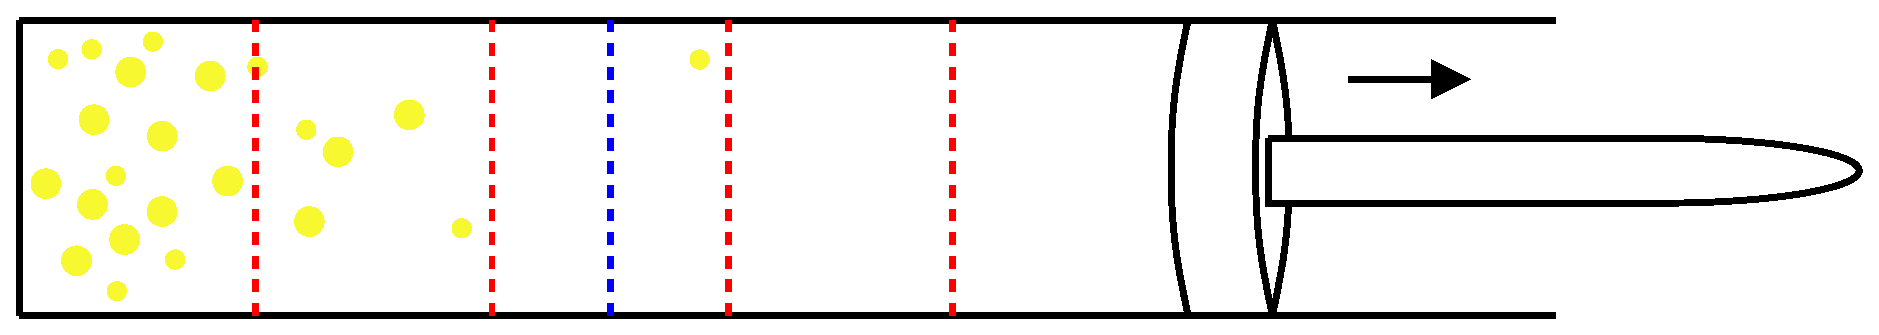
\includegraphics[scale=0.50]{figs/PistonCT.eps}
\caption{Abstract Piston with Representative Partitions: Blue Line for 2 Bins, Red Line for 5 Bins.}
\label{piston_ct}
\end{center}
\end{figure}

Now, to capture the state of the piston, impose imaginary partitions at equidistant points in the chamber.  A diagram of this is seen in Figure \ref{piston_ct}.  The blue
dotted line represents partitioning the piston chamber into two distinct bins.  The particle distribution is heavily weighted to the leftmost bin
since this is where the large majority of the fluid (yellow dots) falls.  

The red dotted lines in Figure \ref{piston_ct} represent the same chamber partitioned into five bins.  The left most red partition runs through the
densely populated region, adding information about the distribution that was not available under the more corasely-binned structure.

From this one might conclude that only an infinite number of partitions and bins would converge 
to the `true' value of the entropy.  However, this is not necessary for contingency tables.  
The metrics (entropy, uncertainty, \emph{et cetera}) rely on the relative populations of the bins.
An infinite number of partitions would result in zero or one particle per bin, thereby giving in poor statistics.

Thus there is a balancing act between the number of bins and the number of stochastic simulation executions.  This study uses a symmetric seven bins per axis formulation.  (Two dimensional tables have $7^2=49$ bins while the three dimensional tables have
$7^3=343$ bins.)
Such behavior is consistent with other Monte Carlo techniques \cite{Press2007}.

\begin{figure}[htbp]
\begin{center}
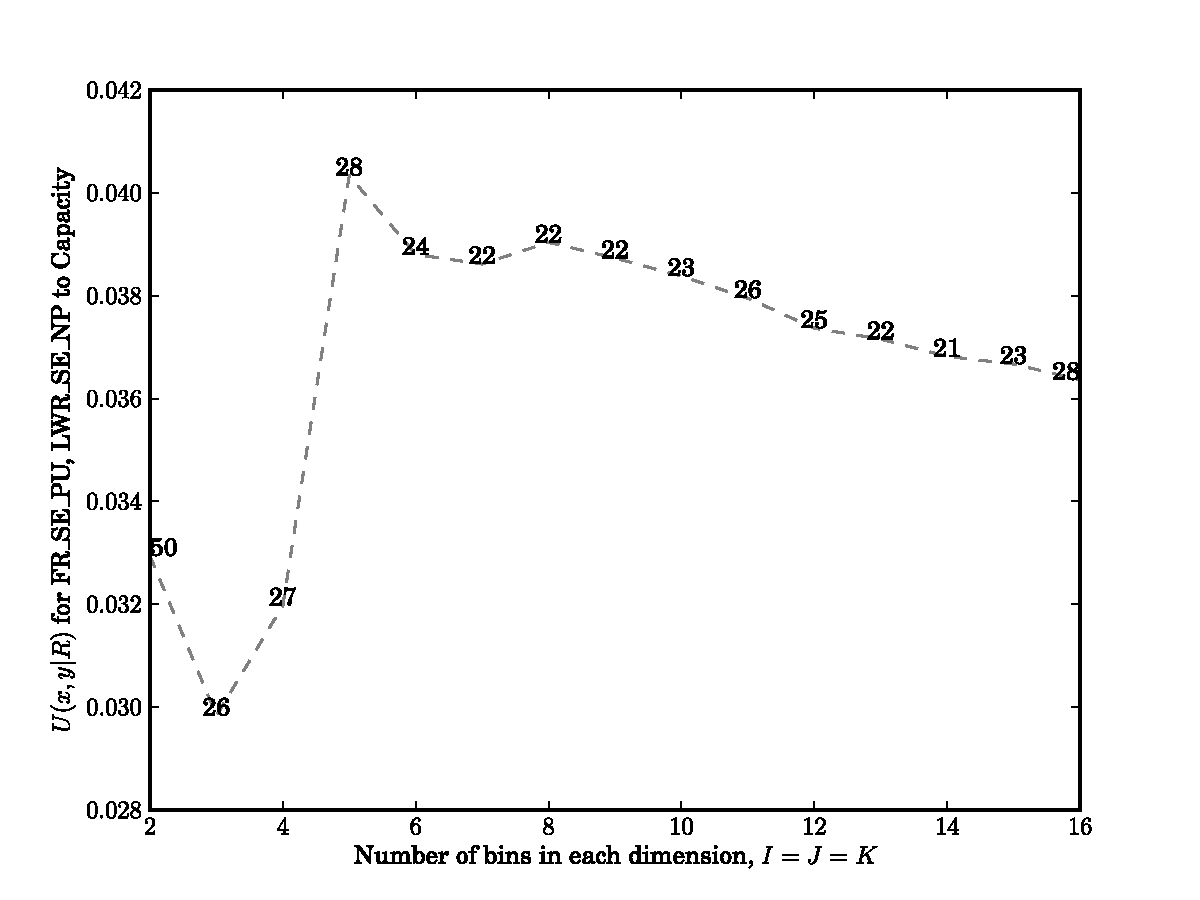
\includegraphics[scale=0.70]{figs/U_xy_R_for_FR_SE_PU_and_LWR_SE_NP_to_Capacity_rank.eps}
\caption{Dynamic Effects of Binning Structure Example: $U(x,y|R)$ for the parameter pair (\texttt{FR\_SE\_PU}, \texttt{LWR\_SE\_NP}) to repository capacity.}
\label{dynamic_effects}
\end{center}
\end{figure}

Seven bins per axis were chosen since the uncertainty rankings for moderately important parameter pairs stabilize at approximately this point.  While the choice of binning resolution is system-specific -- it depends on the dynamics of the underlying simulation model -- important parameters are always going to dominate the top ranks and non-important ones will change ranks rapidly, but randomly.  Therefore it is necessary  to
examine the parameters which are most sensitive to the binning effects.

Figure \ref{dynamic_effects} shows how the 3D sensitivity $U(x,y|R)$ for FR plutonium separation efficiency and LWR neptunium separation efficiency given the repository
capacity changes as a function of symmetric bin structure (\emph{i.e.} $A=B=C$).  It is known that \texttt{FR\_SE\_PU} is very important
while \texttt{LWR\_SE\_NP} is not.  Therefore the combination of these two inputs has some modest impact largely driven by the plutonium vector.

Figure \ref{dynamic_effects} displays both the value of the uncertainty metric for this parameter pair as well as its relative ranking to all other pairs.
Lower ranks ($1, 2, \ldots$) indicate more important parameters while higher ranks ($\ldots, 29, 30$ or $\ldots, 434, 435$) mean that the parameter has less overall
impact.  From this figure, the importance of (\texttt{FR\_SE\_PU}, \texttt{LWR\_SE\_NP}) fluctuates significantly from 50 to the mid-twenties for low symmetric
bin number.  However once 7 bins are reached, the rank stabilizes at ~22.  This stability indicates that the repository capacity response to changes in \texttt{FR\_SE\_PU} and \texttt{LWR\_SE\_NP}, relative to the response for similarly important parameter pairs, becomes well-captured at 7-bin resolution.

After 10 bins, the rank creeps up and down.  This is expected as the number of
fuel cycle realizations remains constant for all bin numbers.  Thus higher bin numbers relate to correspondingly worse statistics for the contingency table (see below).  The goal, therefore, is to pick the lowest bin number after which the rankings have become stable.  Such a point for this study seems to lie at approximately
7 bins per axis.  Studies have been made of several other parameter pairs to support this conclusion.

The mutual information may be used to ensure that the binning structure offers satisfactory statistics given the number of stochastic realizations available.  Since every input parameter is independent of every other input parameter, $I(x,y)$ should be zero for all combinations of $x$ and $y$
in the limit as $N$ becomes large.

Call $t$ the maximum acceptable tolerance along any stochastic axis.
For instance, $t = 0.01$ indicates a 1\% intrinsic uncertainty.
Then the threshold mutual information for `good' statistics goes as $I(x,y) \approx t^2$, since
two stochastic parameters are being compared.  The approximate number of runs required to achieve $t$ is thus:
\begin{equation}
N \approx \frac{1}{t^2} B C
\label{runs_needed}
\end{equation}
Thus by equation \ref{runs_needed}, it is a factor of $25$ times easier to achieve 5\% uncertainty than to get to the 1\% level for the same binning structure.
Given $100,000$ runs performed here and seven bins on each axis, equation \ref{runs_needed} implies
that the induced uncertainty is approximately 2.2\%.  Seven bins per axis are used for the remainder of this analysis.



\subsection{Rankings: One Input to One Response}
\index{Rankings: One Input to One Response@\emph{Rankings: One Input to One Response}}
\label{cts_sec:rank2D}

Determining the impact of a single input parameter on a nuclear fuel cycle outcome is the first step in a screening study.  Using the contingency table methodology above,
the uncertainty coefficient $U(x|R)$ measures the importance of $x$.  Table \ref{U_x_R_for_Capacity_with_IJK7} displays the input parameters, ranked by
uncertainty, for the repository capacity response.

\begin{center}
\begin{table}[htbp]
\caption{Input Parameters Ranked by $U(x|R)$ for \texttt{Capacity} [MTHM/Repository]}
\label{U_x_R_for_Capacity_with_IJK7}\begin{center}
\begin{tabular}{|r|l|c|}
\hline
Rank&\textbf{$x$}&\textbf{$U(x|R)$}\\
\hline
1&\texttt{FR\_SE\_PU}&0.07667\\
\hline
2&\texttt{HLW\_Storage\_Time}&0.05264\\
\hline
3&\texttt{FR\_SE\_AM}&0.04148\\
\hline
4&\texttt{Heat\_Loss\_Factor}&0.01548\\
\hline
5&\texttt{LWR\_SE\_PU}&0.01343\\
\hline
6&\texttt{FR\_TRU\_CR}&0.008895\\
\hline
7&\texttt{LWR\_SE\_AM}&0.007304\\
\hline
8&\texttt{FR\_BUd}&0.003773\\
\hline
9&\texttt{LWR\_SNF\_Storage\_Time}&0.003551\\
\hline
10&\texttt{Rock\_Specific\_Heat}&0.003085\\
\hline
11&\texttt{FR\_SE\_CM}&0.002522\\
\hline
12&\texttt{Rock\_Thermal\_Conductivity}&0.001954\\
\hline
13&\texttt{Ambient\_Temp}&0.001353\\
\hline
14&\texttt{LWR\_BUd}&0.001053\\
\hline
15&\texttt{LWR\_SE\_CS}&0.001033\\
\hline
16&\texttt{LWR\_SE\_SR}&0.001024\\
\hline
17&\texttt{FR\_SNF\_Storage\_Time}&0.0005559\\
\hline
18&\texttt{Drift\_Space}&0.0004421\\
\hline
19&\texttt{LWR\_SE\_U}&0.0002899\\
\hline
20&\texttt{Rock\_Density}&0.0002718\\
\hline
21&\texttt{FR\_SE\_CS}&0.0001331\\
\hline
22&\texttt{FR\_SE\_SR}&0.0001073\\
\hline
23&\texttt{Vent\_System\_On\_Time}&0.0001016\\
\hline
24&\texttt{Drift\_Diameter}&9.648E-05\\
\hline
25&\texttt{LWR\_SE\_NP}&9.575E-05\\
\hline
26&\texttt{LWR\_SE\_CM}&7.969E-05\\
\hline
27&\texttt{LWR\_Fuel2Mod}&7.833E-05\\
\hline
28&\texttt{FR\_LAN\_FF\_Cap}&6.559E-05\\
\hline
29&\texttt{FR\_SE\_NP}&6.212E-05\\
\hline
30&\texttt{FR\_SE\_U}&6.207E-05\\
\hline
\end{tabular}
\end{center}
\end{table}
\end{center}



As expected, the fast reactor plutonium separation efficiency is shown to be the driver of the system.  How much more important this parameter is that the
other inputs may be quantitatively stated by taking the ratio of the two $U(x|R)$.  For instance, \texttt{LWR\_SE\_AM}, the parameter at rank 7,
has an uncertainty of 0.007304.  Meanwhile \texttt{FR\_SE\_PU} has an uncertainty of 0.07667.  The ratio of these uncertainties,
and thus the magnitude of the parameters' effects on relative repository capacity, is 10.5.

From Table \ref{U_x_R_for_Capacity_with_IJK7}, most inputs have at least an order of magnitude less impact than the most important one, \texttt{FR\_SE\_PU}.
This bottom heavy distribution indicates that there are only a handful of fuel cycle parameters which strongly drive
repository capacity over even part of the range on which they are varied.
Namely, they are the LWR \& FR plutonium SE, the HLW storage time, the FR americium SE, and the repository heat loss factor.

However, this only addresses a single response in a large and coupled system.
Similar rankings could be computed in analogy to Table \ref{U_x_R_for_Capacity_with_IJK7} for all other responses.
For example, even fewer inputs were found to be drivers of the LWR/FR support ratio than drive the repository capacity.  The sole parameter above 0.1 uncertainty is, predictably, the fast reactor conversion ratio.
The only two inputs on the range $[0.001, 0.01]$ are the LWR \& FR burnups.  Thus all 27 other inputs are at least two orders of magnitude
less important than the top one for the \texttt{Support\_Ratio}.

Even though the input rankings may change dramatically for different responses, a short list of the most important may be determined from the union of all top
inputs for all response.  Moreover, some responses tend to produce similar rankings because their values are derived from other responses.
This limits the overall number of top parameters.

One non-intuitive result from the 2D study is that the cesium and strontium separation efficiencies do not appear higher in the ranks.  Indeed, the reason for
partitioning these species is \emph{because} of their large impact.  They are ranked relatively low here 
because by the point of 0.9 separations for these species,
the lower bound of the SE range, has been achieved, most of their repository impact has been mitigated.

\subsection{Rankings: Two Inputs to One Response}
\index{Rankings: Two Inputs to One Response@\emph{Rankings: Two Inputs to One Response}}
\label{cts_sec:rank3D}

The analysis of three dimensional contingency tables follows in two parts.  The first is a ranking of associations of input parameter pairs, analogous to
the 2D case.  Second, covariance effects between the two inputs are measured.

\subsubsection{3D Sensitivity}
\index{3D Sensitivity@\emph{3D Sensitivity}}
\label{cts_sec:3D_sensitivity}

%\begin{center}
\begin{table}[htbp]
\caption{Top 10\% Input Parameter Pairs Ranked by $U(x,y|R)$ for \texttt{Capacity} [MTHM/Repository]}
\label{U_xy_R_for_Capacity_with_IJK7}
\begin{center}
\begin{tabular}{|r|l|l|c|}
\hline
Rank&\textbf{$x$}&\textbf{$y$}&\textbf{$U(x,y|R)$}\\
\hline
1&\texttt{FR\_SE\_PU}&\texttt{HLW\_Storage\_Time}&0.07251\\
\hline
2&\texttt{FR\_SE\_AM}&\texttt{FR\_SE\_PU}&0.06461\\
\hline
3&\texttt{FR\_SE\_AM}&\texttt{HLW\_Storage\_Time}&0.05093\\
\hline
4&\texttt{FR\_SE\_PU}&\texttt{Heat\_Loss\_Factor}&0.04923\\
\hline
5&\texttt{FR\_SE\_PU}&\texttt{LWR\_SE\_PU}&0.04637\\
\hline
6&\texttt{FR\_SE\_PU}&\texttt{FR\_TRU\_CR}&0.0447\\
\hline
7&\texttt{FR\_SE\_PU}&\texttt{LWR\_SE\_AM}&0.04275\\
\hline
8&\texttt{FR\_BUd}&\texttt{FR\_SE\_PU}&0.04153\\
\hline
9&\texttt{FR\_SE\_PU}&\texttt{LWR\_SNF\_Storage\_Time}&0.0411\\
\hline
10&\texttt{FR\_SE\_PU}&\texttt{Rock\_Specific\_Heat}&0.04055\\
\hline
11&\texttt{FR\_SE\_CM}&\texttt{FR\_SE\_PU}&0.04019\\
\hline
12&\texttt{FR\_SE\_PU}&\texttt{Rock\_Thermal\_Conductivity}&0.0399\\
\hline
13&\texttt{FR\_SE\_PU}&\texttt{LWR\_BUd}&0.03947\\
\hline
14&\texttt{Ambient\_Temp}&\texttt{FR\_SE\_PU}&0.03946\\
\hline
15&\texttt{FR\_SE\_PU}&\texttt{LWR\_SE\_SR}&0.0392\\
\hline
16&\texttt{FR\_SE\_PU}&\texttt{LWR\_SE\_CS}&0.03916\\
\hline
17&\texttt{FR\_SE\_PU}&\texttt{FR\_SNF\_Storage\_Time}&0.03899\\
\hline
18&\texttt{Drift\_Space}&\texttt{FR\_SE\_PU}&0.0389\\
\hline
19&\texttt{FR\_SE\_PU}&\texttt{Rock\_Density}&0.03875\\
\hline
20&\texttt{FR\_SE\_PU}&\texttt{LWR\_SE\_U}&0.03874\\
\hline
21&\texttt{FR\_SE\_NP}&\texttt{FR\_SE\_PU}&0.03862\\
\hline
22&\texttt{FR\_SE\_PU}&\texttt{LWR\_SE\_NP}&0.03862\\
\hline
23&\texttt{FR\_SE\_PU}&\texttt{LWR\_SE\_CM}&0.03861\\
\hline
24&\texttt{FR\_SE\_PU}&\texttt{FR\_SE\_SR}&0.0386\\
\hline
25&\texttt{FR\_LAN\_FF\_Cap}&\texttt{FR\_SE\_PU}&0.0386\\
\hline
26&\texttt{FR\_SE\_CS}&\texttt{FR\_SE\_PU}&0.03859\\
\hline
27&\texttt{Drift\_Diameter}&\texttt{FR\_SE\_PU}&0.03859\\
\hline
28&\texttt{FR\_SE\_PU}&\texttt{LWR\_Fuel2Mod}&0.03859\\
\hline
29&\texttt{FR\_SE\_PU}&\texttt{FR\_SE\_U}&0.03859\\
\hline
30&\texttt{FR\_SE\_PU}&\texttt{Vent\_System\_On\_Time}&0.03857\\
\hline
31&\texttt{Heat\_Loss\_Factor}&\texttt{HLW\_Storage\_Time}&0.03595\\
\hline
32&\texttt{HLW\_Storage\_Time}&\texttt{LWR\_SE\_PU}&0.03457\\
\hline
33&\texttt{FR\_TRU\_CR}&\texttt{HLW\_Storage\_Time}&0.03158\\
\hline
34&\texttt{HLW\_Storage\_Time}&\texttt{LWR\_SNF\_Storage\_Time}&0.03113\\
\hline
35&\texttt{HLW\_Storage\_Time}&\texttt{LWR\_SE\_AM}&0.03091\\
\hline
36&\texttt{FR\_SE\_AM}&\texttt{Heat\_Loss\_Factor}&0.0301\\
\hline
37&\texttt{FR\_SE\_CM}&\texttt{HLW\_Storage\_Time}&0.02929\\
\hline
38&\texttt{FR\_BUd}&\texttt{HLW\_Storage\_Time}&0.02872\\
\hline
39&\texttt{FR\_SE\_AM}&\texttt{LWR\_SE\_PU}&0.02842\\
\hline
40&\texttt{HLW\_Storage\_Time}&\texttt{Rock\_Specific\_Heat}&0.02829\\
\hline
41&\texttt{HLW\_Storage\_Time}&\texttt{LWR\_SE\_CS}&0.02804\\
\hline
42&\texttt{HLW\_Storage\_Time}&\texttt{LWR\_SE\_SR}&0.02783\\
\hline
43&\texttt{HLW\_Storage\_Time}&\texttt{Rock\_Thermal\_Conductivity}&0.02771\\
\hline
44&\texttt{FR\_SE\_AM}&\texttt{FR\_TRU\_CR}&0.02746\\
\hline
\end{tabular}
\end{center}
\end{table}
\end{center}


The three dimensional expression of the uncertainty coefficient, $U(x,y|R)$, is used to capture the strength of association from a parameter pair to the response.
Therefore a table similar to Table \ref{U_x_R_for_Capacity_with_IJK7} would show the rankings of all 435 parameter pairs
to the repository capacity.

However, from the previous 2D study, the \texttt{FR\_SE\_PU}
is known to be the most important single parameter to repository capacity by a wide margin.  Because of this overwhelming impact, \texttt{FR\_SE\_PU} appears as a member of
29 of the top 30 pairs in the 3D sensitivity study.  In fact, the only pair in the top thirty which does not contain FR plutonium SE is the rank 3 pair
(\texttt{FR\_SE\_AM}, \texttt{HLW\_Storage\_Time}), which simply matches the rank 2 \& 3 inputs from the two-dimensional contingency tables.
Thus if an input is important by its own merits, any pair that this input is a member of is likely to also have a large system-wide effect.
Since little additional information is added here over the 2D study, the specific 3D sensitivity tables are not displayed.

\subsubsection{3D Sensitivity of Sensitivity}
\index{3D Sensitivity of Sensitivity@\emph{3D Sensitivity of Sensitivity}}
\label{cts_sec:3D_sensitivity_of_sensitivity}

As was seen in section \ref{sec:3D_sensitivity}, the three dimensional uncertainty coefficient did not reveal fundamentally different information
about the system than the two dimensional rankings.  $U(x,y|R)$ coupled important inputs together, but which inputs were important remained the same.  This was
due to the fact that inputs were still being measured against a response.

How one input affects the impact of another input is a critical issue to the system designer.  For example, one would want to know that the gains made by
changing the \texttt{FR\_SE\_PU} would thrust another, previously unimportant, system design parameter to the fore.  As a second example, if \texttt{HLW\_Storage\_Time} and \texttt{LWR\_UF\_Storage\_Time} are seen to have a strong joint effect, it may mean that pursuing a strategy of extensive pre-emplacement storage would require lengthier pre-separation used fuel storage to be most effective.

\begin{center}
\begin{table}[htbp]
\caption{Top 10\% Input Parameter Pairs Ranked by $c_v(x|y|R)$ for \texttt{Capacity} [MTHM/Repository]}
\label{cv_x_y_R_for_Capacity_with_IJK7}
\begin{center}
\begin{tabular}{|r|l|l|c|}
\hline
Rank&\textbf{$x$}&\textbf{$y$}&\textbf{$c_v(x|y|R)$}\\
\hline
1&\texttt{FR\_SE\_AM}&\texttt{HLW\_Storage\_Time}&0.02318\\
\hline
2&\texttt{FR\_SE\_AM}&\texttt{FR\_SE\_PU}&0.02316\\
\hline
3&\texttt{HLW\_Storage\_Time}&\texttt{LWR\_UF\_Storage\_Time}&0.01557\\
\hline
4&\texttt{FR\_SE\_PU}&\texttt{HLW\_Storage\_Time}&0.01556\\
\hline
5&\texttt{HLW\_Storage\_Time}&\texttt{LWR\_SE\_PU}&0.01155\\
\hline
6&\texttt{FR\_SE\_AM}&\texttt{FR\_TRU\_CR}&0.01061\\
\hline
7&\texttt{FR\_SE\_PU}&\texttt{LWR\_UF\_Storage\_Time}&0.008192\\
\hline
8&\texttt{FR\_SE\_PU}&\texttt{LWR\_SE\_PU}&0.008\\
\hline
9&\texttt{FR\_BUd}&\texttt{FR\_SE\_AM}&0.007716\\
\hline
10&\texttt{Ambient\_Temp}&\texttt{FR\_SE\_PU}&0.007489\\
\hline
11&\texttt{Ambient\_Temp}&\texttt{HLW\_Storage\_Time}&0.007367\\
\hline
12&\texttt{HLW\_Storage\_Time}&\texttt{LWR\_SE\_AM}&0.007248\\
\hline
13&\texttt{Ambient\_Temp}&\texttt{FR\_SE\_CS}&0.007235\\
\hline
14&\texttt{Ambient\_Temp}&\texttt{LWR\_Fuel2Mod}&0.007066\\
\hline
15&\texttt{Ambient\_Temp}&\texttt{Heat\_Loss\_Factor}&0.007044\\
\hline
16&\texttt{Ambient\_Temp}&\texttt{Rock\_Specific\_Heat}&0.007013\\
\hline
17&\texttt{Ambient\_Temp}&\texttt{FR\_SE\_NP}&0.00698\\
\hline
18&\texttt{Ambient\_Temp}&\texttt{Drift\_Diameter}&0.006958\\
\hline
19&\texttt{Ambient\_Temp}&\texttt{FR\_SE\_AM}&0.006935\\
\hline
20&\texttt{Ambient\_Temp}&\texttt{LWR\_SE\_PU}&0.006906\\
\hline
21&\texttt{FR\_SE\_CM}&\texttt{HLW\_Storage\_Time}&0.006894\\
\hline
22&\texttt{Ambient\_Temp}&\texttt{LWR\_SE\_CS}&0.006864\\
\hline
23&\texttt{Ambient\_Temp}&\texttt{Drift\_Space}&0.006842\\
\hline
24&\texttt{Ambient\_Temp}&\texttt{FR\_SE\_U}&0.006839\\
\hline
25&\texttt{Ambient\_Temp}&\texttt{FR\_SE\_CM}&0.006795\\
\hline
26&\texttt{Ambient\_Temp}&\texttt{FR\_SE\_SR}&0.006792\\
\hline
27&\texttt{Ambient\_Temp}&\texttt{FR\_LAN\_FF\_Cap}&0.006775\\
\hline
28&\texttt{Ambient\_Temp}&\texttt{LWR\_SE\_CM}&0.006773\\
\hline
29&\texttt{Ambient\_Temp}&\texttt{LWR\_SE\_AM}&0.006763\\
\hline
30&\texttt{Ambient\_Temp}&\texttt{LWR\_SE\_U}&0.006726\\
\hline
31&\texttt{Ambient\_Temp}&\texttt{LWR\_BUd}&0.006714\\
\hline
32&\texttt{Ambient\_Temp}&\texttt{FR\_UF\_Storage\_Time}&0.006704\\
\hline
33&\texttt{Ambient\_Temp}&\texttt{LWR\_SE\_SR}&0.006695\\
\hline
34&\texttt{Ambient\_Temp}&\texttt{Rock\_Density}&0.006676\\
\hline
35&\texttt{Ambient\_Temp}&\texttt{FR\_BUd}&0.006667\\
\hline
36&\texttt{Ambient\_Temp}&\texttt{LWR\_SE\_NP}&0.006663\\
\hline
37&\texttt{Ambient\_Temp}&\texttt{Vent\_System\_On\_Time}&0.006651\\
\hline
38&\texttt{Ambient\_Temp}&\texttt{Rock\_Thermal\_Conductivity}&0.006595\\
\hline
39&\texttt{Ambient\_Temp}&\texttt{FR\_TRU\_CR}&0.006588\\
\hline
40&\texttt{Ambient\_Temp}&\texttt{LWR\_UF\_Storage\_Time}&0.006544\\
\hline
41&\texttt{FR\_BUd}&\texttt{FR\_SE\_PU}&0.006506\\
\hline
42&\texttt{HLW\_Storage\_Time}&\texttt{LWR\_SE\_CS}&0.006502\\
\hline
43&\texttt{FR\_SE\_CM}&\texttt{FR\_SE\_PU}&0.006427\\
\hline
44&\texttt{FR\_SE\_PU}&\texttt{FR\_TRU\_CR}&0.006298\\
\hline
\end{tabular}
\end{center}
\end{table}
\end{center}



These sensitivities of sensitivities are measured in terms of the coefficient of variation $c_v$, as described in section \ref{sec:sensitivity_of_sensitivity_metrics}.
Table \ref{cv_x_y_R_for_Capacity_with_IJK7} shows the top 10\% of 435 ranked parameter pairs for $c_v(x|y|R)$ for the repository capacity.
As expected, the top parameters from before (\texttt{FR\_SE\_PU}, \texttt{FR\_SE\_AM}, \& \texttt{HLW\_Storage\_Time}) all exhibit large effects on
the impact of the others.

An input that is present in most of the top pairs in Table \ref{cv_x_y_R_for_Capacity_with_IJK7} is the
ambient environment temperature of the repository.
In many cases, this makes intuitive sense.  The majority of the inputs that \texttt{Ambient\_Temp} is paired with here are those that affect the composition of
material in the repository (\emph{i.e.} the various SE, the FR conversion ratio, the LWR fuel to moderator ratio).
Moreover, the \texttt{Ambient\_Temp} itself may be seen as a metric of remaining heat capacity in the repository while the material composition determines the heat load.
Thus the fact that such parameters pairs exhibit strong covariances is not surprising.



\subsection{Case Studies}
\index{Case Studies@\emph{Case Studies}}
\label{cts_sec:case_studies}

\subsubsection{Covariance of Plutonium \& Americium Separations}
\index{Covariance of Plutonium \& Americium Separations@\emph{Covariance of Plutonium \& Americium Separations}}
\label{cts_sec:pu_am_se}

Plutonium and americium separation efficiencies provide an intuitive example of the covariance measure.  There is already known
to be a strong coupling between these two parameters with respect to the repository capacity \cite{Scopatz2009c}.  From the
2D sensitivity study, both \texttt{FR\_SE\_PU} and \texttt{FR\_SE\_AM} are highly ranked inputs.  They exhibit
a high covariance because \nuc{Pu}{238} and \nuc{Am}{241} are in direct competition for being the top heat load contributor to the
repository.  Therefore, the degree to which plutonium is recycled in the FR relative to that of americium shifts
repository performance in a way that may have a greater impact than when altering \texttt{FR\_SE\_PU} and \texttt{FR\_SE\_AM}
in tandem.

\begin{figure}[htbp]
\begin{center}
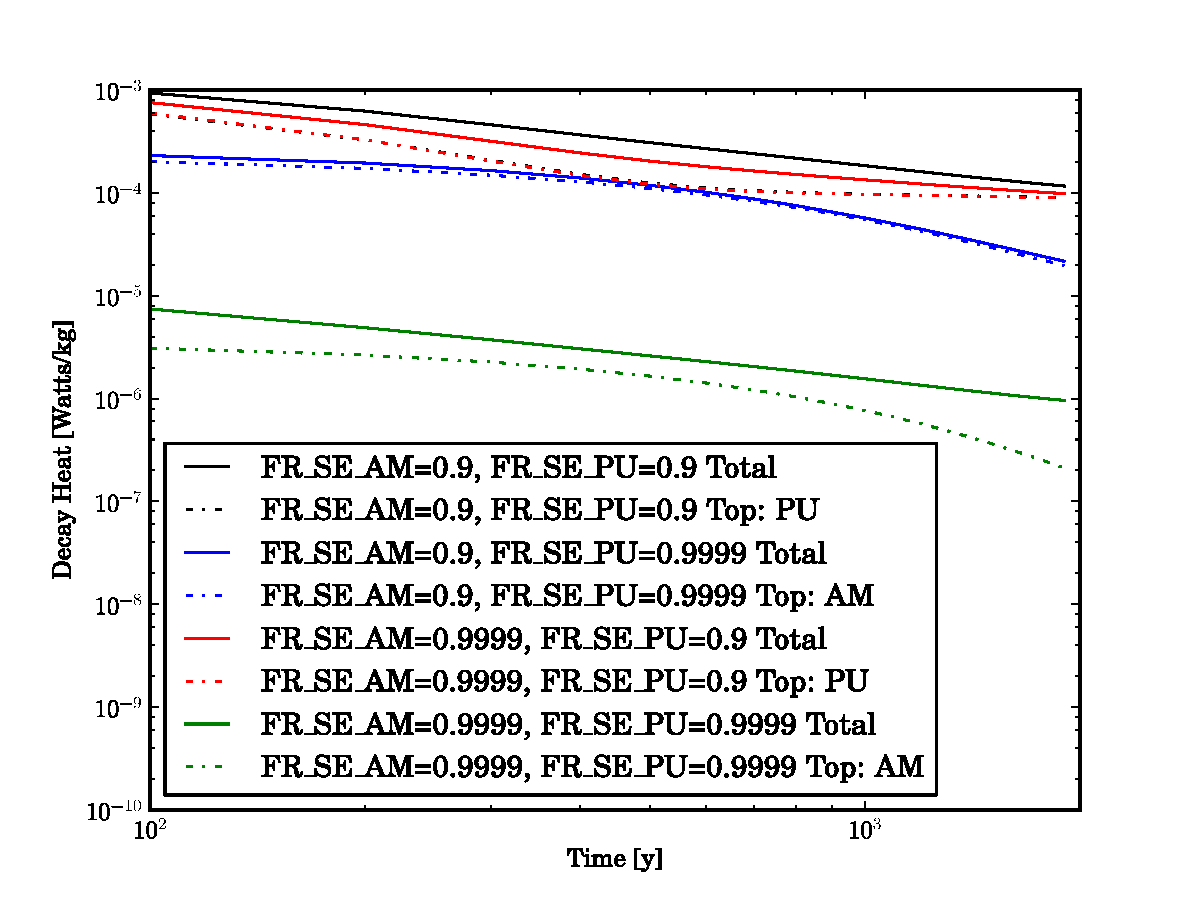
\includegraphics[scale=0.70]{figs/FR_SE_AM_and_FR_SE_PU_Decay_Heat.eps}
\caption{Total \& Top Contibutor Decay Heat [Watts/kg] of HLW for the parameter pair (\texttt{FR\_SE\_AM}, \texttt{FR\_SE\_PU}).}
\label{am_pu_decay_heat}
\end{center}
\end{figure}

Such covariant effects are visible in Figure \ref{am_pu_decay_heat}.
Low values of \texttt{FR\_SE\_PU} and \texttt{FR\_SE\_AM} have high decay heats and high values have low decay heats.
However, for the middle cases where one parameter is high and one is low, the top contributor takes on the value of the low separation efficiency.
The switch between Am/Pu and the two order of magnitude range in the decay heat is captured by the covariance metric.


\subsubsection{Covariance of Americium Separations and FR TRU Conversion Ratio}
\index{Covariance of Americium Separations and FR TRU Conversion Ratio@\emph{Covariance of Americium Separations and FR TRU Conversion Ratio}}
\label{cts_sec:am_se_fr_tru_cr}

The interplay between the FR americium SE and the FR transuranic conversion ratio exhibits a covariance
to the repository capacity.  As seen in Table \ref{cv_x_y_R_for_Capacity_with_IJK7}, these two inputs display a relatively high sensitivity of sensitivity.  The covariance effect here is confirmed by examining Table \ref{FR_SE_AM_and_FR_TRU_CR_to_Capacity_with_IJK433_prop}.

\begin{center}
\begin{table}[htbp]
\caption{Probability Table for FR Americium Separation Efficiency \& FR Transuranic Conversion Ratio to Repository Capacity [MTHM/Repository].}
\label{FR_SE_AM_and_FR_TRU_CR_to_Capacity_with_IJK433_prop}
%\scriptsize
\tiny
\begin{center}
\begin{tabular}{|c||c|c|c||c|}
\hline
\multicolumn{5}{|c|}{Slice for 0.25 $<$ \texttt{FR\_TRU\_CR} $<$ 0.483}\\
\hline
&$0.9 <$ \texttt{FR\_SE\_AM} $< 0.99$&$0.99 <$ \texttt{FR\_SE\_AM} $< 0.999$&$0.999 <$ \texttt{FR\_SE\_AM} $< 0.9999$&\\
\hline
$10^4 <$ \texttt{Capacity} $< 10^5$&2.10E-04&7.63E-05&5.72E-05&3.43E-04\\
\hline
$10^5 <$ \texttt{Capacity} $< 10^6$&8.94E-02&6.31E-02&5.97E-02&2.12E-01\\
\hline
$10^6 <$ \texttt{Capacity} $< 10^7$&2.14E-02&4.70E-02&4.71E-02&1.15E-01\\
\hline
$10^7 <$ \texttt{Capacity} $< 10^8$&1.91E-05&1.46E-03&4.12E-03&5.60E-03\\
\hline
&1.11E-01&1.12E-01&1.11E-01&3.34E-01\\
\hline
\hline
\multicolumn{5}{|c|}{Slice for 0.483 $<$ \texttt{FR\_TRU\_CR} $<$ 0.717}\\
\hline
&$0.9 <$ \texttt{FR\_SE\_AM} $< 0.99$&$0.99 <$ \texttt{FR\_SE\_AM} $< 0.999$&$0.999 <$ \texttt{FR\_SE\_AM} $< 0.9999$&\\
\hline
$10^4 <$ \texttt{Capacity} $< 10^5$&1.14E-03&4.20E-04&3.43E-04&1.90E-03\\
\hline
$10^5 <$ \texttt{Capacity} $< 10^6$&9.68E-02&7.09E-02&6.64E-02&2.34E-01\\
\hline
$10^6 <$ \texttt{Capacity} $< 10^7$&1.22E-02&4.01E-02&4.10E-02&9.33E-02\\
\hline
$10^7 <$ \texttt{Capacity} $< 10^8$&0.00E-00&7.25E-04&2.79E-03&3.51E-03\\
\hline
&1.10E-01&1.12E-01&1.11E-01&3.33E-01\\
\hline
\hline
\multicolumn{5}{|c|}{Slice for 0.717 $<$ \texttt{FR\_TRU\_CR} $<$ 0.95}\\
\hline
&$0.9 <$ \texttt{FR\_SE\_AM} $< 0.99$&$0.99 <$ \texttt{FR\_SE\_AM} $< 0.999$&$0.999 <$ \texttt{FR\_SE\_AM} $< 0.9999$&\\
\hline
$10^4 <$ \texttt{Capacity} $< 10^5$&3.37E-03&1.05E-03&1.06E-03&5.48E-03\\
\hline
$10^5 <$ \texttt{Capacity} $< 10^6$&1.02E-01&7.49E-02&6.92E-02&2.46E-01\\
\hline
$10^6 <$ \texttt{Capacity} $< 10^7$&6.00E-03&3.46E-02&3.84E-02&7.90E-02\\
\hline
$10^7 <$ \texttt{Capacity} $< 10^8$&0.00E-00&2.29E-04&2.74E-03&2.97E-03\\
\hline
&1.11E-01&1.11E-01&1.11E-01&3.33E-01\\
\hline
\hline
\multicolumn{5}{|c|}{Summary for summation over \texttt{FR\_TRU\_CR}}\\
\hline
&$0.9 <$ \texttt{FR\_SE\_AM} $< 0.99$&$0.99 <$ \texttt{FR\_SE\_AM} $< 0.999$&$0.999 <$ \texttt{FR\_SE\_AM} $< 0.9999$&\\
\hline
$10^4 <$ \texttt{Capacity} $< 10^5$&4.71E-03&1.55E-03&1.46E-03&7.72E-03\\
\hline
$10^5 <$ \texttt{Capacity} $< 10^6$&2.88E-01&2.09E-01&1.95E-01&6.92E-01\\
\hline
$10^6 <$ \texttt{Capacity} $< 10^7$&3.96E-02&1.22E-01&1.26E-01&2.88E-01\\
\hline
$10^7 <$ \texttt{Capacity} $< 10^8$&1.91E-05&2.41E-03&9.64E-03&1.21E-02\\
\hline
&3.33E-01&3.35E-01&3.33E-01&1.00E+00\\
\hline
\end{tabular}
\end{center}
\end{table}
\end{center}





Table \ref{FR_SE_AM_and_FR_TRU_CR_to_Capacity_with_IJK433_prop} displays the probability table, which is a normalized representation of the contingency table.
This table shows that repository capacity increases with increasing \texttt{FR\_SE\_AM}, a result consistent
with the previous case study.  On the other hand, with increasing \texttt{FR\_TRU\_CR}, the repository capacity \emph{decreases}.  Moreover, the
peak of the repository capacity distribution as a function
of americium separations increases with increasing \texttt{FR\_TRU\_CR}.

This covariance effect is due in part to the fact that the \texttt{FR\_TRU\_CR} is the major driver of the support ratio.  As the conversion ratio
increases, the mass of LWR UF required per kilogram of FR fresh fuel decreases.  Therefore all components downstream from the FR become correspondingly more important;
there are simply fewer LWRs.  In specific, the relative impact of \texttt{FR\_SE\_AM} increases.

Due to increasing \texttt{FR\_TRU\_CR}, the americium contribution (as measured through \nuc{Am}{241}) negatively affects the repository capacity.  At high conversion ratios, there is more high Am content FR UF per unit nuclear electricity produced.  This in turn implies that the
packing density of used fuel per meter of drift tunnel goes down.  Therefore the total mass of heavy metal (\texttt{Capacity}) that may be stored in a
fixed-size repository decreases.


\subsubsection{Covariance of HLW Storage Time \& Fast Reactor Plutonium Separations}
\index{Covariance of HLW Storage Time \& Fast Reactor Plutonium Separations@\emph{Covariance of HLW Storage Time \& Fast Reactor Plutonium Separations}}
\label{cts_sec:hlw_pu_covariance}

The top two inputs from the sensitivity study, \texttt{FR\_SE\_PU} and \texttt{HLW\_Storage\_Time}, appear to exert a strong joint effect on the outcome.  According to Table \ref{cv_x_y_R_for_Capacity_with_IJK7}, this input pair is ranked fifth with respect to $c_v(x|y|R)$.
Through an examination of the the 3D contingency table, high respository capacities are only allowed when both \texttt{FR\_SE\_PU} and
\texttt{HLW\_Storage\_Time} are high.  Similarly, low capacities occur for low values of the two inputs.  Middle values for either of the
inputs yield middling capacities.  Additionally, the entropy increases with increasing \texttt{FR\_SE\_PU} and \texttt{HLW\_Storage\_Time}.

\begin{figure}[htbp]
\begin{center}
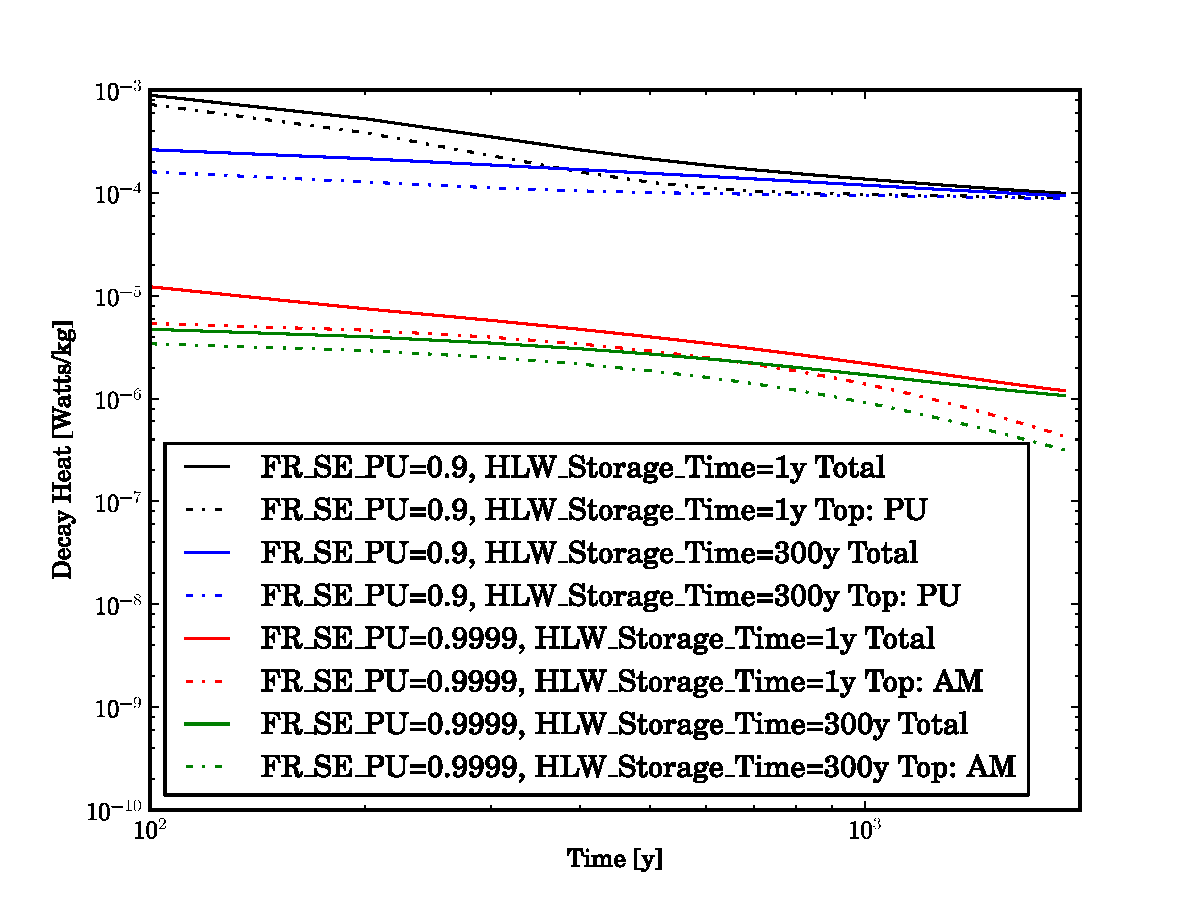
\includegraphics[scale=0.70]{figs/FR_SE_PU_and_HLW_Storage_Time_Decay_Heat.eps}
\caption{Total \& Top Contibutor Decay Heat [Watts/kg] of HLW for the parameter pair (\texttt{HLW\_Storage\_Time}, \texttt{FR\_SE\_PU}).}
\label{hlw_pu_decay_heat}
\end{center}
\end{figure}

Physically, the reason for this covariance is because the HLW storage time effectively shifts the opening time of the repository.
By having a long \texttt{HLW\_Storage\_Time}, the short- and medium-term repository tempurature limits may be avoided.
Figure \ref{hlw_pu_decay_heat} displays the decay heat for the HLW and for the top elemental contributor to the decay heat as a
function of time after emplacement in the repository.  The curves here represent the four corner cases of the input values.

The time shift effect may be observed by holding \texttt{FR\_SE\_PU} constant and comparing curves on Figure \ref{hlw_pu_decay_heat}
where \texttt{HLW\_Storage\_Time} is one year to the curves where the storage time is three hundred years.  Points on the 1 year curves have
roughly the same value as the 300 year HLW storage time curves, only 300 years farther in the future.  By shifting the 1 year data
three hundred years to the left, the two curves would nearly overlap.  The statistical analysis confirms the strong importance to repository capacity of a strategy of `waiting out' the decay of Pu-238 if Pu separation efficiencies are low, and its much weaker importance if efficiencies are high.

\section{Concluding Remarks \& Future Work}
\index{Concluding Remarks \& Future Work@\emph{Concluding Remarks \& Future Work}}
\label{cts_sec:conclusion}

The statistical techniques of contingency table and entropy analysis presented in this paper are widely-used tools for capturing the behavior of complex systems, particularly biological ones.  Here they have been applied to a simulator of the nuclear fuel cycle.  NFC outcomes, like those of any complex system, are shaped by intricate and highly nonlinear interactions between many inputs.

The strength of association between the inputs and the outcome studied here, the capacity of a Yucca Mountain-like repository, was quantified through uncertainty coefficients.  Three-dimensional uncertainties were augmented by a coefficient of variation to determine the system response inputs acting jointly.  The latter is especially important because alternative approaches, for instance linear sensitivity analyses, can only capture the response to departures from a reference state.  This reference state is defined by the values assumed by dozens or hundreds of system inputs, each of which may be varied by system or technology designers.  It was shown that the coefficient of variation could illuminate dependencies where changes in one input have a strong effect on the system response to another.  

This tool can aid system designers by helping them perceive which design variables matter.  The contingency tables represent a (coarsely-gridded) importance map for the inverse problem.  Conditioned on a specific system response, like repository capacity, the measure of the strength of response provided by the uncertainty coefficients can provide guidance to technologists optimizing design parameters in the face of uncertainty regarding the shape of the larger system.  Illuminating joint dependencies, coefficients of variation can guide iterative technology development by showing which design features must be considered together.

The approach described here can be generalized to include boolean as well as continuous inputs.  For example, if the technology ultimately chosen for the permanent repository is unknown, a boolean flag can allow each stochastic realization to follow one of several options.  The outcome, still repository capacity, would now be conditioned on this boolean input as well.  It would illuminate system design parameters that will be important regardless of technology ultimately chosen, those that have strongly technology-dependent effects, and those that are unimportant to determining capacity regardless of technology.  In view of the uncertainties in the direction taken by nuclear energy in the future, coupled with the need to develop technologies now that can support or even enable these outcomes, this capability, if developed, could provide invaluable guidance.
